\documentclass{article}


\usepackage{arxiv}

\usepackage[utf8]{inputenc} % allow utf-8 input
\usepackage[T1]{fontenc}    % use 8-bit T1 fonts
\usepackage{hyperref}       % hyperlinks
\usepackage{url}            % simple URL typesetting
\usepackage{booktabs}       % professional-quality tables
\usepackage{amsfonts}       % blackboard math symbols
\usepackage{nicefrac}       % compact symbols for 1/2, etc.
\usepackage{microtype}      % microtypography
\usepackage{lipsum}
\usepackage{graphicx}
\graphicspath{ {./images/} }


\title{Event Classification for Higgs Particle with Quantum Machine Learning in 
      High-Energy Physics}


\author{
 Shiwen An \\
  School of High Energy Accelerator Science\\
  The Graduate University for Advanced Studies, SOKENDAI\\
  Tsukuba, Japan \\
  \texttt{shiwenan@post.kek.jp} \\
  %% examples of more authors
   \And
  Xuanqiang Zhao \\
  Department of Computer Science\\
  University of Hong Kong\\
  HK \\
  \texttt{Xuanqiang.Zhao@hku.edu} \\
  %% \AND
  %% Coauthor \\
  %% Affiliation \\
  %% Address \\
  %% \texttt{email} \\
  %% \And
  %% Coauthor \\
  %% Affiliation \\
  %% Address \\
  %% \texttt{email} \\
  %% \And
  %% Coauthor \\
  %% Affiliation \\
  %% Address \\
  %% \texttt{email} \\
}

\begin{document}
\maketitle
\begin{abstract}
Machine Learning Algorithms like Deep Neural Network (DNN), Binary Decision Tree (BDT), has been used in 
high energy physics for a long time, specifically in track signal identification and supervised classification tasks. 
Meanwhile, quantum computing was proposed by Richard Feynman in the early 1980s as a way to performs computations that 
would be unreachable by classical computers. Over the past 40 years, the noisy intermediate-scale quantum computing 
devices have been developed and multiple new algorithms are proposed with such device. In this paper, we present the 
studies of quantum algorithms exploiting machine learning to classify the events of interest from background.
\end{abstract}


% keywords can be removed
\keywords{ Quantum Machine Learning \and Variational Quantum Circuit \and Variational Shadow Quantum Learning \and Quantum Kernel Method\and }


\section{Introduction}
In High-Energy Physics experiments, particles created by collisions are observed by layers of high precision detectors.
In this field, many early attempts to use quantum computing for HEP exist. For example, the data analysis \cite{qml_task1}, identification
of charged particles[], reconstruction of particles collision points []. ([] indicates adding citation based on those paper) As discussed in 
many literatures, the quantum machine learning (QML) is considered as one of the QC algorithms that could bring quantum 
advantages over classical methods[\cite{qml_icepp}, 16].

\section{Task description and data construction}
Discrimination of events of interests is always the most frequently used ML techniques in HEP data analysis. 
In this research, we examine the most frequently used variational quantum classider (VQC), Quantum Kernel Methods, 
Variational Shadow Quantum Learning (VSQL) \cite{qml_vsql} and Quantum Generative Adversarial Network (Quantum GAN). 
\label{sec:headings}
\paragraph{Dataset} Here we use the dataset from UCI's Machine Learning Repository [\href{https://archive.ics.uci.edu/ml/datasets/HIGGS}{Lib}]. 
\paragraph{Task modeling.}
We approach this task as a regression problem. For every item and shop pair, we need to predict its next month sales(a number).
\paragraph{Construct train and test data.}
The dataset provided has 28 features, 21 low-level features and 7 high-level features. 

\subsection{Method 1: Variational Quantum Classifier}

\subsection{Method 2: Variational Shadow Quantum Learning}

\subsection(Method 3: Variational Shadow Quantum Learning)
\lipsum[6]

\paragraph{Paragraph}
\lipsum[7]

\section{Examples of citations, figures, tables, references}
\label{sec:others}
\lipsum[8] \cite{kour2014real,kour2014fast} and see \cite{hadash2018estimate}.

The documentation for \verb+natbib+ may be found at
\begin{center}
  \url{http://mirrors.ctan.org/macros/latex/contrib/natbib/natnotes.pdf}
\end{center}
Of note is the command \verb+\citet+, which produces citations
appropriate for use in inline text.  For example,
\begin{verbatim}
   \citet{hasselmo} investigated\dots
\end{verbatim}
produces
\begin{quote}
  Hasselmo, et al.\ (1995) investigated\dots
\end{quote}

\begin{center}
  \url{https://www.ctan.org/pkg/booktabs}
\end{center}


\subsection{Figures}
\lipsum[10] 
See Figure \ref{fig:fig1}. Here is how you add footnotes. \footnote{Sample of the first footnote.}
\lipsum[11] 

\begin{figure}
  \centering
  \fbox{\rule[-.5cm]{4cm}{4cm} \rule[-.5cm]{4cm}{0cm}}
  \caption{Sample figure caption.}
  \label{fig:fig1}
\end{figure}

\begin{figure} % picture
    \centering
    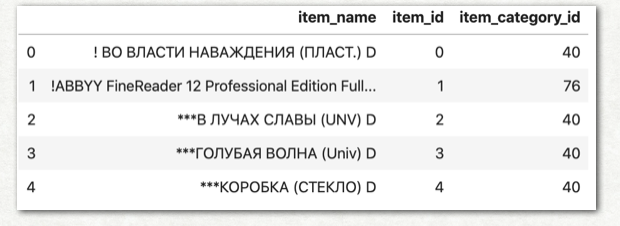
\includegraphics{test.png}
\end{figure}

\subsection{Tables}
\lipsum[12]
See awesome Table~\ref{tab:table}.

\begin{table}
 \caption{Sample table title}
  \centering
  \begin{tabular}{lll}
    \toprule
    \multicolumn{2}{c}{Part}                   \\
    \cmidrule(r){1-2}
    Name     & Description     & Size ($\mu$m) \\
    \midrule
    Dendrite & Input terminal  & $\sim$100     \\
    Axon     & Output terminal & $\sim$10      \\
    Soma     & Cell body       & up to $10^6$  \\
    \bottomrule
  \end{tabular}
  \label{tab:table}
\end{table}

\subsection{Lists}
\begin{itemize}
\item Lorem ipsum dolor sit amet
\item consectetur adipiscing elit. 
\item Aliquam dignissim blandit est, in dictum tortor gravida eget. In ac rutrum magna.
\end{itemize}


\bibliographystyle{unsrt}  
%\bibliography{references}  %%% Remove comment to use the external .bib file (using bibtex).
%%% and comment out the ``thebibliography'' section.


%%% Comment out this section when you \bibliography{references} is enabled.
\begin{thebibliography}{1}

\bibitem{qml_icepp}

\bibitem{qml_vsql}
Li, G., Song, Z., \& Wang, X. (2021). 
VSQL: Variational Shadow Quantum Learning for Classification. 
Proceedings of the AAAI Conference on Artificial Intelligence, 35(9), 8357-8365. \url{https://doi.org/10.1609/aaai.v35i9.17016}

\bibitem{qml_task1}
Mott, A., Job, J., Vlimant, JR. et al. Solving a Higgs optimization problem with 
quantum annealing for machine learning. Nature 550, 375–379 (2017). \url{https://doi.org/10.1038/nature24047}

\bibitem{kour2014real}
George Kour and Raid Saabne.
\newblock Real-time segmentation of on-line handwritten arabic script.
\newblock In {\em Frontiers in Handwriting Recognition (ICFHR), 2014 14th
  International Conference on}, pages 417--422. IEEE, 2014.

\bibitem{kour2014fast}
George Kour and Raid Saabne.
\newblock Fast classification of handwritten on-line arabic characters.
\newblock In {\em Soft Computing and Pattern Recognition (SoCPaR), 2014 6th
  International Conference of}, pages 312--318. IEEE, 2014.

\bibitem{hadash2018estimate}
Guy Hadash, Einat Kermany, Boaz Carmeli, Ofer Lavi, George Kour, and Alon
  Jacovi.
\newblock Estimate and replace: A novel approach to integrating deep neural
  networks with existing applications.
\newblock {\em arXiv preprint arXiv:1804.09028}, 2018.

\end{thebibliography}


\end{document}
